%=================================================================
\chapter{CASO DE ESTUDIO}  \label{cha:studycase}
%=================================================================

El presente framework ha sido aplicado en el Instituto Colombiano para la Evaluaci\'on de la Educaci\'on (ICFES) \cite{icfes:2012}, entidad especializada y encargada por ley de la evaluaci\'on en todos los niveles de la educaci\'on en Colombia. El ICFES tiene dentro de sus funciones: Desarrollar la fundamentaci\'on te\'orica, dise\~nar, elaborar y aplicar instrumentos de evaluaci\'on a la poblaci\'on objetivo, y publicar los resultados de estas evaluaciones a la comunidad educativa.

Para el cumplimiento de su misi\'on el Instituto tiene definidos procesos de negocio como: Registrar los usuarios a cada una de las pruebas ofrecidas. Dise\~nar y construir los instrumentos de evaluaci\'on (cuestionarios de papel) que permiten medir las competencias y componentes de los evaluados. Aplicar estos instrumentos a toda la poblaci\'on en una fecha determinada. Calificar y publicar los resultados obtenidos tanto a nivel individual como agrupado (por instituci\'on educativa). Tanto los procesos de negocio como las entidades de datos del ICFES est\'an descritos en espa\~nol, por temas de confidencialidad las descripciones de los elementos de BA e IA fueron traducidas al idioma Ingl\'es.
%........................................................

\begin{figure}[!t]
\begin{center}
	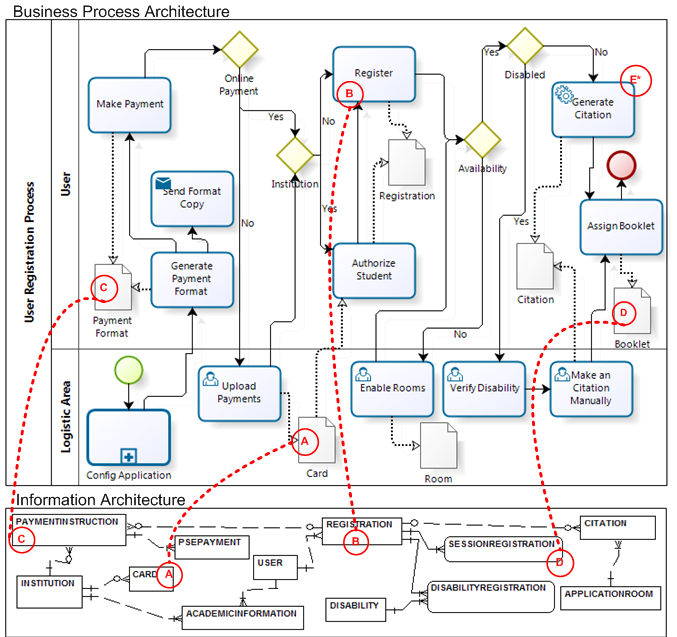
\includegraphics[scale=0.6 ,natwidth=669pt, natheight=637pt]{BA-IA_mapp.png}
	\caption{Diagrama BPMN del Proceso User Registration y su esquema S1}
	\label{fig:BA-IA}
\end{center}
\end{figure} 

%........................................................

Para ilustrar nuestra propuesta nos vamos a enfocar en dos procesos: \textit{User Registration} y \textit{Corporate User Registration}. El proceso \textit{User Registration} se detalla en la Figura \ref{fig:BA-IA}, el dominio de negocio se describe utilizando Business Process Management Notation (BPMN) y el Modelo Entidad Relaci\'on estructura los elementos que conforman el dominio de informaci\'on (esquema \texttt{S1}). Este proceso es uno de los principales en la vertical de negocio y es cr\'itico dado que cada usuario (un mill\'on al an\~o aproximadamente) crea una instancia de este proceso. Adem\'as debe ser afinado o ajustado en cada aplicaci\'on (seis veces al a\~no). En cuanto a la IA, el esquema de base de datos (\texttt{S1}) que soporta \textit{User Registration} apoya adem\'as otros procesos misionales y por tanto est\'a compuesto por mas de 200 tablas, de las cuales hemos extra\'ido solo las que nos ayudan a ejemplificar nuestro caso de estudio. Con el prop\'osito de determinar el grado en el que este proceso de negocio es soportado por los datos (alineaci\'on BA-IA), un arquitecto debe realizar una revisi\'on manual de estos diagramas, apoyado en artefactos adicionales como: Descripci\'on detallada de los procesos y diccionario de datos. 

Estas revisiones son la entrada para hallar las correspondencias (trazas) entre IA y BA, para lo cual un arquitecto debe realizar diversas comparaciones.

La comparaci\'on \textit{textual} consiste en contrastar cadenas de caracteres (mapeos A y B en la Figura \ref{fig:BA-IA}). En el caso el mapeo C implica hallar similitudes \textit{lig\"u\'isticas} que se apoyen en sin\'onimos e hiper\'onimos. Por otro lado, hay correspondencias m\'as complejas de identificar como es el caso de \texttt{BOOKLET} (Mapeo D) que a simple vista no parece ser soportado por ninguna entidad. Sin embargo revisando el diccionario de datos en detalle, se encuentra el campo \texttt{SESSIONREGISTRATION.BOOKLETNUMBER} el cual almacena el n\'umero de cuadernillo del usuario. 

Adicionalmente, inferir redundancias dentro de cada dominio conlleva, por un lado a contrastar todos los elementos de los procesos dentro la BA, y por el otro, comparar todas las entidades de los esquemas al interior de la IA. Tomemos por ejemplo el otro proceso de negocio del ICFES llamado \textit{Corporate User Registration} cuyo diagrama BPMN est\'a descrito en la Figura \ref{fig:LightRegistering}. Este proceso es soportado por el esquema \texttt{S2} y soporta la inscripci\'on de usuarios a evaluaciones contratadas por clientes corporativos. Tiene similitudes con el proceso anterior, dado que incluye la carga de inscritos, generaci\'on de citaci\'on y cuadernillos, pero es mas liviano, menos restrictivo y menos automatizado. El proceso de \texttt{Corporate User Registration} no ofrece inscripci\'on en l\'inea, no requiere de un pago individual para inscribirse, pero presenta actividades con similitudes sem\'anticas con respecto a \textit{User Registration}. Por ejemplo  \textit{Register} y \textit{Migrate Registered} (B y B$^{\ast}$) o la actividad \textit{Generate Citation} que esta presente en ambos procesos (E y E$^{\ast}$). A nivel de datos, tambi\'en es clave conocer posibles entidades redundantes como \texttt{REGISTRATION} en \texttt{S1} (B) e \texttt{REGISTERED} en \texttt{S2} (B$^{\ast}$).

%--------------------------------------------------------------------------------------
\begin{figure}[!t]
\begin{center}
	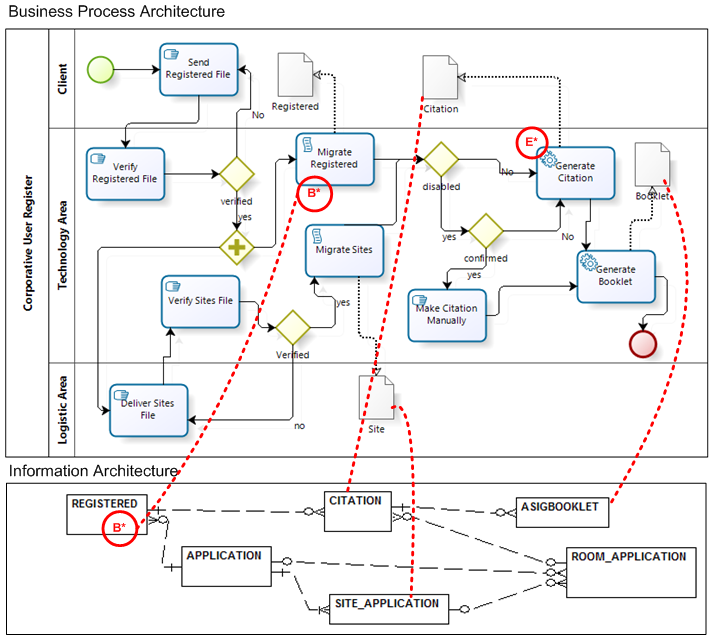
\includegraphics[scale=0.5 ,natwidth=713pt, natheight=635pt]{LightRegistering.PNG}
	\caption{Diagrama BPMN del Proceso Coporative User Registration y el esquema S2}
	\label{fig:LightRegistering}
\end{center}
\end{figure} 
%--------------------------------------------------------------------------------------

El total de comparaciones de alineaci\'on est\'a dado por el producto cartesiano ($M \times N$), donde $M$ es la cantidad de elementos de $BA$ y $N$ la cantidad de elementos de $IA$. La cantidad de verificaciones de redundancia est\'a dada por el coeficiente binomial $\frac{{n!}}{2!(n-2)!}$, donde $n$ es la cantidad de elementos a contrastar en cada dominio ($M$ o $N$).

Para dimensionar la cantidad de comparaciones a realizar de forma exhaustiva, tomemos como ejemplo el segmento de la EA del ICFES comprendido por los procesos y esquemas abordados en este cap\'itulo. La BA est\'a compuesta por dos procesos de negocio (21 actividades) y la IA est\'a compuesta por dos esquemas (18 tablas). La tarea de definir la trazabilidad (comparar todos los elementos BA-IA) implica ejecutar 378 comparaciones. Sumado a esto, la evaluaci\'on de redundancias implicar\'ia 210 verificaciones en BA y 153 en IA. En total, se necesitar\'ian 741 comprobaciones para evaluar las heur\'isticas de alineamiento propuestas en el Cap\'itulo \ref{cha:intro}. Lo que implica un tedioso y costoso trabajo manual sobre solo dos procesos de negocio y sin tener en cuenta los atributos de las entidades y los elementos de los procesos de negocio diferentes a las actividades (i. e. Gateways, Events, Subprocess). 
